%
%  progress-presentation.tex
%  src
%
%  Created by Illya Starikov on 09/16/17.
%  Copyright 2017. Illya Starikov. All rights reserved.
%

% \documentclass[notes,xcolor=dvipsnames]{beamer}       % print frame + notes
% \documentclass[notes=only,xcolor=dvipsnames]{beamer}  % only notes
\documentclass[xclolor=dvipsnames]{beamer}            % only frames
%\documentclass[handout,xclolor=dvipsnames]{beamer}    % only frames, no pauses
\usepackage{soul,graphics}

\usepackage{amssymb,amsmath,verbatim,graphicx,microtype,upquote,units,booktabs,akkwidepage}

\newcommand{\chapterNumber}[1]{
    \setcounter{section}{#1}
    \addtocounter{section}{-1}
}
\title{Observation (Presentation \#7)}
\subtitle{Special Topics (CS3001)}
\author{Illya Starikov}
\date{Sometimes In The Future}
\institute{Missouri University of Science and Technology}

\begin{document}
\begin{darkframes}
    \maketitle

    \begin{frame}
        \frametitle{Backstory}

        At the beginning of the semester, one of my friends got me into the television Psych. Spoiler lies ahead. If you don't want to be spoiled, simply watch the first episode (it's on Amazon Prime Video).

    \end{frame}

    \begin{frame}
        \frametitle{Backstory}

        \begin{figure}[H]
            \centering
            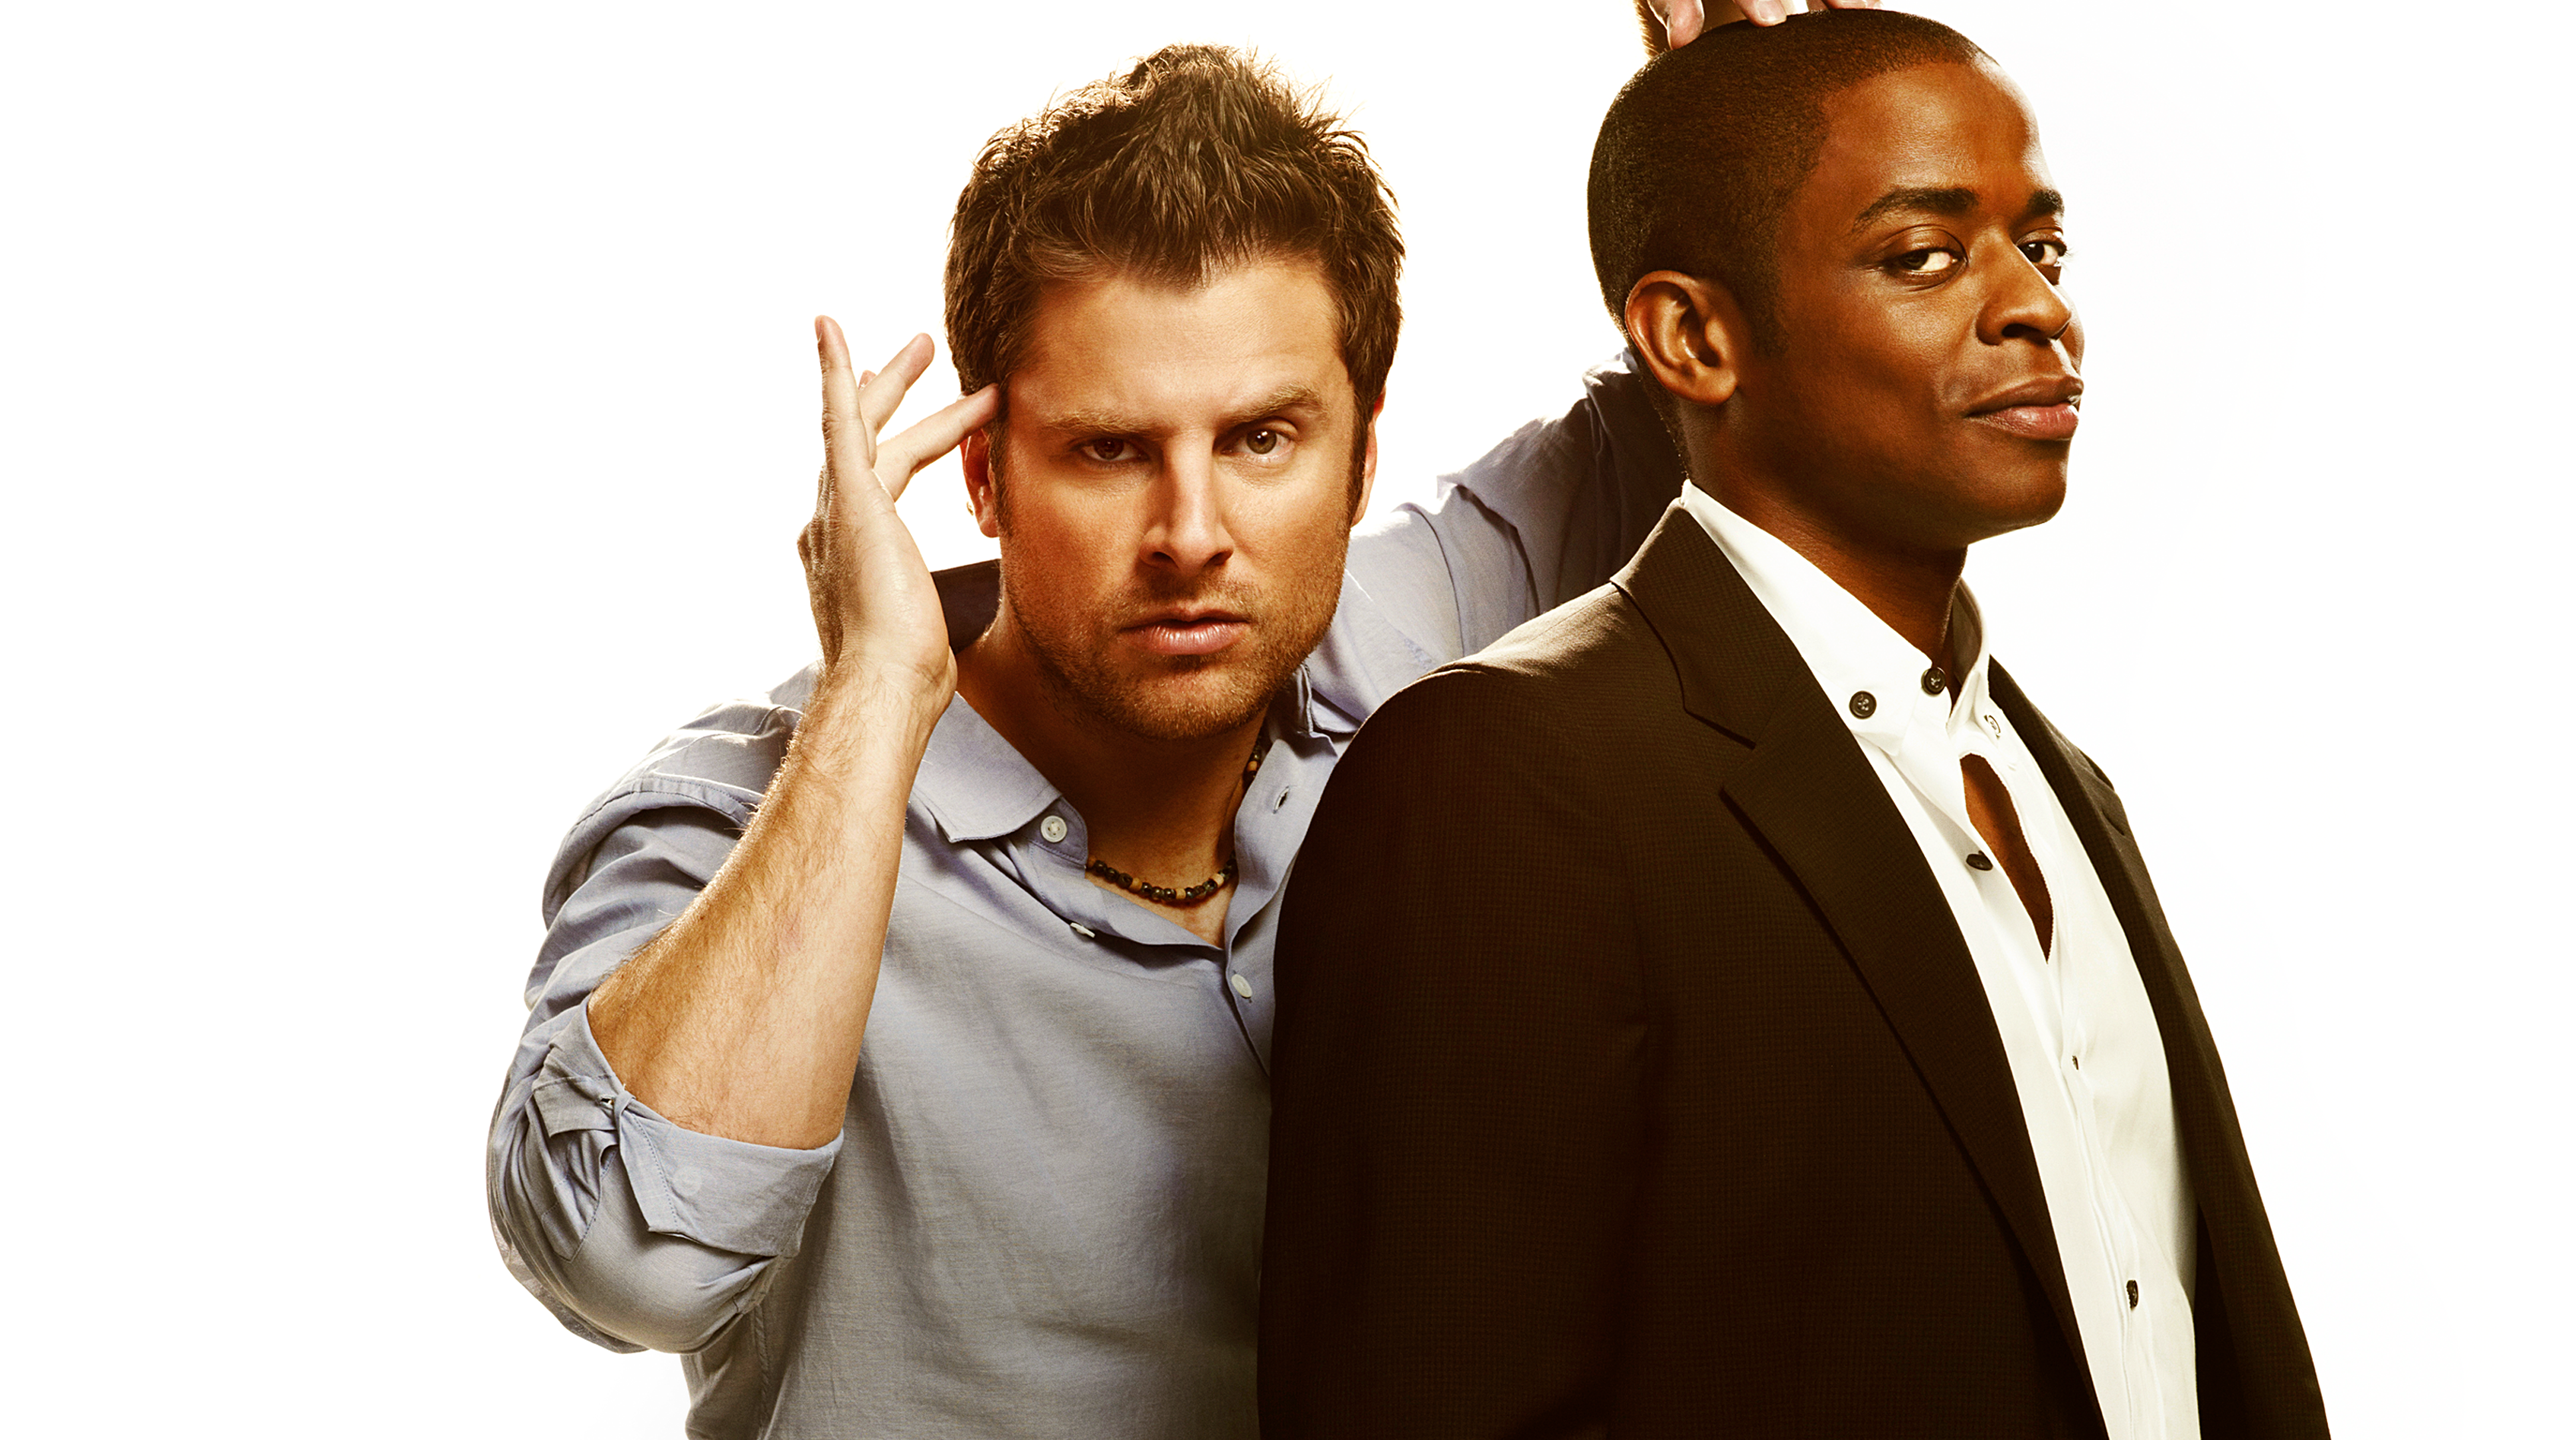
\includegraphics[width=.9\linewidth]{assets/psych.png}
            \caption{The Psych Sitcom}
            \label{fig:psych}
        \end{figure}

    \end{frame}

    \begin{frame}
        \frametitle{Backstory}

        The basic premise of Psych is thus: there is an extremely observant protagonist that pretends to be psychic. His ``Psychic visions'' are simply conclusions he draws from details he observes. I took note of the exceptional attention to detail he paid, and wanted to emulate this in my everyday life.

    \end{frame}

    \begin{frame}
        \frametitle{Goals}

        \begin{itemize}
            \item The goal of becoming more observant were difficult to describe.
            \item I wanted to generally go by feeling.
                \begin{itemize}
                    \item Some days I feel as if I was very observant, other days I felt as if I was not very observant.
                \end{itemize}
        \end{itemize}
    \end{frame}


    \begin{frame}
        \frametitle{Actions Taken}
        I started generally paying attention to things, such as:

        \begin{itemize}
            \item What people wear
            \item Their mannerism
            \item What would make them upset
            \item What would make them happy
        \end{itemize}

        I would even try to test my ability to pay attention by trying to memorize license plates on my way walking to class, and trying to see how many I was able to recognize on my way back from class (generally a five hour delay).
    \end{frame}


    \begin{frame}
        \frametitle{Resources}

        \begin{itemize}
            \item I read one book on the subject: \href{https://www.amazon.com/What-Every-BODY-Saying-Speed-Reading/dp/B006ZNFEKW}{What Every BODY Saying}
            \item Other than that, a lot of the resources were the people I observed.
        \end{itemize}
    \end{frame}

    \begin{frame}
        \frametitle{Goal Accomplishment}

        \begin{itemize}
            \item I feel as if I have become a lot more observant this semester.
            \item However, this is a skill that does leave when you don't use it.
            \item I want to continually practice this the rest of my life.
        \end{itemize}
    \end{frame}

    \begin{frame}
        \frametitle{An Example}

        A couple of my roommates and I were out at the bar. When we went outside, I noticed a man smoking a cigarette. Using my observational ability, I notice near the filter of the cigarette it said ``Marlboro'', and I noticed his drink was something with coke. Using my deducing ability, I started off a conservation with him with ``Marlboro/Rum and Coke I see''. He responsed, with astonishment, ``Are you physic?''.

    \end{frame}

    \begin{frame}
        \frametitle{In Closing}

        All question, comments, and insults can be directed towards me:

        \begin{center}
            \begin{description}
                \item[\faComment] \href{mailto:starikov@mst.edu}{starikov@mst.edu}
                \item[\faLinkedin] \href{https://www.linkedin.com/in/illyastarikov/}{Illya Starikov}
                \item[\faGithub] \href{https://github.com/IllyaStarikov/}{Illya Starikov}
                \item[\faRss] \href{https://freneticarray.com/}{FreneticArray.com}
            \end{description}
        \end{center}

    \end{frame}
\end{darkframes}
\end{document}
